% Created by tikzDevice version 0.12.6 on 2025-11-06 20:50:23
% !TEX encoding = UTF-8 Unicode
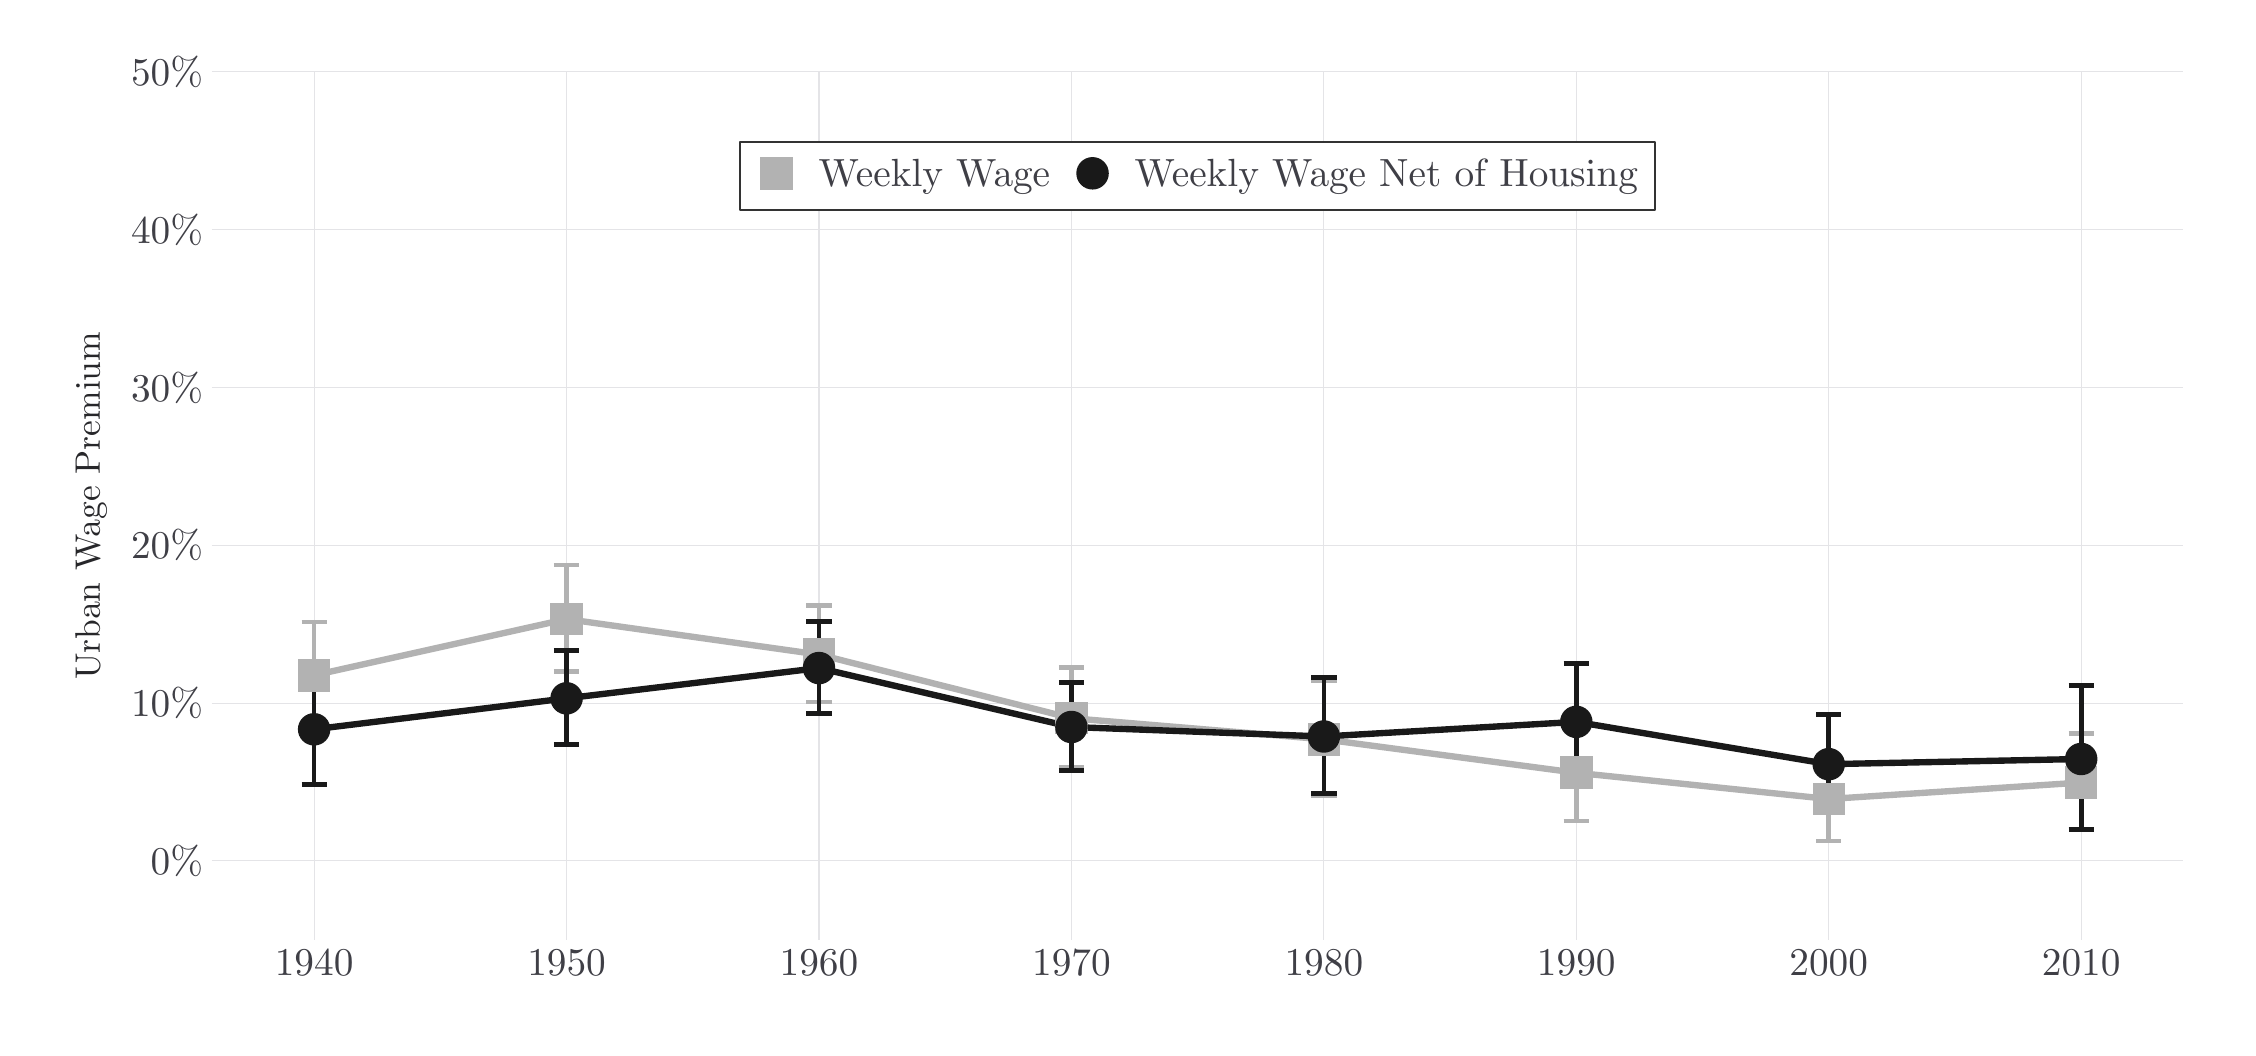
\begin{tikzpicture}[x=1pt,y=1pt]
\definecolor{fillColor}{RGB}{255,255,255}
\path[use as bounding box,fill=fillColor] (0,0) rectangle (794.97,361.35);
\begin{scope}
\path[clip] (  0.00,  0.00) rectangle (794.97,361.35);
\definecolor{drawColor}{RGB}{255,255,255}

\path[draw=drawColor,line width= 0.8pt,line join=round,line cap=round,fill=fillColor] (  0.00,  0.00) rectangle (794.97,361.35);
\end{scope}
\begin{scope}
\path[clip] ( 66.57, 31.76) rectangle (778.97,345.35);
\definecolor{drawColor}{RGB}{255,255,255}
\definecolor{fillColor}{RGB}{255,255,255}

\path[draw=drawColor,line width= 0.8pt,line join=round,line cap=round,fill=fillColor] ( 66.57, 31.76) rectangle (778.97,345.35);
\definecolor{drawColor}{RGB}{228,228,231}

\path[draw=drawColor,line width= 0.4pt,line join=round] ( 66.57, 60.27) --
	(778.97, 60.27);

\path[draw=drawColor,line width= 0.4pt,line join=round] ( 66.57,117.28) --
	(778.97,117.28);

\path[draw=drawColor,line width= 0.4pt,line join=round] ( 66.57,174.30) --
	(778.97,174.30);

\path[draw=drawColor,line width= 0.4pt,line join=round] ( 66.57,231.32) --
	(778.97,231.32);

\path[draw=drawColor,line width= 0.4pt,line join=round] ( 66.57,288.33) --
	(778.97,288.33);

\path[draw=drawColor,line width= 0.4pt,line join=round] ( 66.57,345.35) --
	(778.97,345.35);

\path[draw=drawColor,line width= 0.4pt,line join=round] (103.51, 31.76) --
	(103.51,345.35);

\path[draw=drawColor,line width= 0.4pt,line join=round] (194.73, 31.76) --
	(194.73,345.35);

\path[draw=drawColor,line width= 0.4pt,line join=round] (285.94, 31.76) --
	(285.94,345.35);

\path[draw=drawColor,line width= 0.4pt,line join=round] (377.16, 31.76) --
	(377.16,345.35);

\path[draw=drawColor,line width= 0.4pt,line join=round] (468.38, 31.76) --
	(468.38,345.35);

\path[draw=drawColor,line width= 0.4pt,line join=round] (559.59, 31.76) --
	(559.59,345.35);

\path[draw=drawColor,line width= 0.4pt,line join=round] (650.81, 31.76) --
	(650.81,345.35);

\path[draw=drawColor,line width= 0.4pt,line join=round] (742.03, 31.76) --
	(742.03,345.35);
\definecolor{drawColor}{gray}{0.70}

\path[draw=drawColor,line width= 2.3pt,line join=round] (103.51,127.34) --
	(194.73,147.64) --
	(285.94,134.83) --
	(377.16,111.83) --
	(468.38,104.20) --
	(559.59, 92.11) --
	(650.81, 82.63) --
	(742.03, 88.57);
\definecolor{drawColor}{gray}{0.10}

\path[draw=drawColor,line width= 2.3pt,line join=round] (103.51,107.82) --
	(194.73,119.01) --
	(285.94,129.94) --
	(377.16,108.64) --
	(468.38,105.22) --
	(559.59,110.50) --
	(650.81, 95.21) --
	(742.03, 97.09);
\definecolor{drawColor}{gray}{0.70}

\path[draw=drawColor,line width= 1.7pt,line join=round] ( 98.95,146.64) --
	(108.07,146.64);

\path[draw=drawColor,line width= 1.7pt,line join=round] (103.51,146.64) --
	(103.51,108.60);

\path[draw=drawColor,line width= 1.7pt,line join=round] ( 98.95,108.60) --
	(108.07,108.60);
\definecolor{drawColor}{gray}{0.10}

\path[draw=drawColor,line width= 1.7pt,line join=round] ( 98.95,128.51) --
	(108.07,128.51);

\path[draw=drawColor,line width= 1.7pt,line join=round] (103.51,128.51) --
	(103.51, 87.80);

\path[draw=drawColor,line width= 1.7pt,line join=round] ( 98.95, 87.80) --
	(108.07, 87.80);
\definecolor{drawColor}{gray}{0.70}

\path[draw=drawColor,line width= 1.7pt,line join=round] (190.17,167.15) --
	(199.29,167.15);

\path[draw=drawColor,line width= 1.7pt,line join=round] (194.73,167.15) --
	(194.73,128.69);

\path[draw=drawColor,line width= 1.7pt,line join=round] (190.17,128.69) --
	(199.29,128.69);
\definecolor{drawColor}{gray}{0.10}

\path[draw=drawColor,line width= 1.7pt,line join=round] (190.17,136.28) --
	(199.29,136.28);

\path[draw=drawColor,line width= 1.7pt,line join=round] (194.73,136.28) --
	(194.73,102.21);

\path[draw=drawColor,line width= 1.7pt,line join=round] (190.17,102.21) --
	(199.29,102.21);
\definecolor{drawColor}{gray}{0.70}

\path[draw=drawColor,line width= 1.7pt,line join=round] (281.38,152.45) --
	(290.50,152.45);

\path[draw=drawColor,line width= 1.7pt,line join=round] (285.94,152.45) --
	(285.94,117.67);

\path[draw=drawColor,line width= 1.7pt,line join=round] (281.38,117.67) --
	(290.50,117.67);
\definecolor{drawColor}{gray}{0.10}

\path[draw=drawColor,line width= 1.7pt,line join=round] (281.38,146.67) --
	(290.50,146.67);

\path[draw=drawColor,line width= 1.7pt,line join=round] (285.94,146.67) --
	(285.94,113.63);

\path[draw=drawColor,line width= 1.7pt,line join=round] (281.38,113.63) --
	(290.50,113.63);
\definecolor{drawColor}{gray}{0.70}

\path[draw=drawColor,line width= 1.7pt,line join=round] (372.60,130.12) --
	(381.72,130.12);

\path[draw=drawColor,line width= 1.7pt,line join=round] (377.16,130.12) --
	(377.16, 94.06);

\path[draw=drawColor,line width= 1.7pt,line join=round] (372.60, 94.06) --
	(381.72, 94.06);
\definecolor{drawColor}{gray}{0.10}

\path[draw=drawColor,line width= 1.7pt,line join=round] (372.60,124.72) --
	(381.72,124.72);

\path[draw=drawColor,line width= 1.7pt,line join=round] (377.16,124.72) --
	(377.16, 92.96);

\path[draw=drawColor,line width= 1.7pt,line join=round] (372.60, 92.96) --
	(381.72, 92.96);
\definecolor{drawColor}{gray}{0.70}

\path[draw=drawColor,line width= 1.7pt,line join=round] (463.82,125.39) --
	(472.94,125.39);

\path[draw=drawColor,line width= 1.7pt,line join=round] (468.38,125.39) --
	(468.38, 83.72);

\path[draw=drawColor,line width= 1.7pt,line join=round] (463.82, 83.72) --
	(472.94, 83.72);
\definecolor{drawColor}{gray}{0.10}

\path[draw=drawColor,line width= 1.7pt,line join=round] (463.82,126.44) --
	(472.94,126.44);

\path[draw=drawColor,line width= 1.7pt,line join=round] (468.38,126.44) --
	(468.38, 84.71);

\path[draw=drawColor,line width= 1.7pt,line join=round] (463.82, 84.71) --
	(472.94, 84.71);
\definecolor{drawColor}{gray}{0.70}

\path[draw=drawColor,line width= 1.7pt,line join=round] (555.03,110.07) --
	(564.15,110.07);

\path[draw=drawColor,line width= 1.7pt,line join=round] (559.59,110.07) --
	(559.59, 74.68);

\path[draw=drawColor,line width= 1.7pt,line join=round] (555.03, 74.68) --
	(564.15, 74.68);
\definecolor{drawColor}{gray}{0.10}

\path[draw=drawColor,line width= 1.7pt,line join=round] (555.03,131.67) --
	(564.15,131.67);

\path[draw=drawColor,line width= 1.7pt,line join=round] (559.59,131.67) --
	(559.59, 90.04);

\path[draw=drawColor,line width= 1.7pt,line join=round] (555.03, 90.04) --
	(564.15, 90.04);
\definecolor{drawColor}{gray}{0.70}

\path[draw=drawColor,line width= 1.7pt,line join=round] (646.25, 98.24) --
	(655.37, 98.24);

\path[draw=drawColor,line width= 1.7pt,line join=round] (650.81, 98.24) --
	(650.81, 67.42);

\path[draw=drawColor,line width= 1.7pt,line join=round] (646.25, 67.42) --
	(655.37, 67.42);
\definecolor{drawColor}{gray}{0.10}

\path[draw=drawColor,line width= 1.7pt,line join=round] (646.25,113.13) --
	(655.37,113.13);

\path[draw=drawColor,line width= 1.7pt,line join=round] (650.81,113.13) --
	(650.81, 77.80);

\path[draw=drawColor,line width= 1.7pt,line join=round] (646.25, 77.80) --
	(655.37, 77.80);
\definecolor{drawColor}{gray}{0.70}

\path[draw=drawColor,line width= 1.7pt,line join=round] (737.47,106.25) --
	(746.59,106.25);

\path[draw=drawColor,line width= 1.7pt,line join=round] (742.03,106.25) --
	(742.03, 71.40);

\path[draw=drawColor,line width= 1.7pt,line join=round] (737.47, 71.40) --
	(746.59, 71.40);
\definecolor{drawColor}{gray}{0.10}

\path[draw=drawColor,line width= 1.7pt,line join=round] (737.47,123.67) --
	(746.59,123.67);

\path[draw=drawColor,line width= 1.7pt,line join=round] (742.03,123.67) --
	(742.03, 71.63);

\path[draw=drawColor,line width= 1.7pt,line join=round] (737.47, 71.63) --
	(746.59, 71.63);
\definecolor{fillColor}{gray}{0.70}

\path[fill=fillColor] ( 97.64,121.47) --
	(109.38,121.47) --
	(109.38,133.21) --
	( 97.64,133.21) --
	cycle;
\definecolor{fillColor}{gray}{0.10}

\path[fill=fillColor] (103.51,107.82) circle (  5.87);
\definecolor{fillColor}{gray}{0.70}

\path[fill=fillColor] (188.85,141.77) --
	(200.60,141.77) --
	(200.60,153.51) --
	(188.85,153.51) --
	cycle;
\definecolor{fillColor}{gray}{0.10}

\path[fill=fillColor] (194.73,119.01) circle (  5.87);
\definecolor{fillColor}{gray}{0.70}

\path[fill=fillColor] (280.07,128.96) --
	(291.82,128.96) --
	(291.82,140.70) --
	(280.07,140.70) --
	cycle;
\definecolor{fillColor}{gray}{0.10}

\path[fill=fillColor] (285.94,129.94) circle (  5.87);
\definecolor{fillColor}{gray}{0.70}

\path[fill=fillColor] (371.29,105.95) --
	(383.03,105.95) --
	(383.03,117.70) --
	(371.29,117.70) --
	cycle;
\definecolor{fillColor}{gray}{0.10}

\path[fill=fillColor] (377.16,108.64) circle (  5.87);
\definecolor{fillColor}{gray}{0.70}

\path[fill=fillColor] (462.50, 98.33) --
	(474.25, 98.33) --
	(474.25,110.08) --
	(462.50,110.08) --
	cycle;
\definecolor{fillColor}{gray}{0.10}

\path[fill=fillColor] (468.38,105.22) circle (  5.87);
\definecolor{fillColor}{gray}{0.70}

\path[fill=fillColor] (553.72, 86.24) --
	(565.47, 86.24) --
	(565.47, 97.99) --
	(553.72, 97.99) --
	cycle;
\definecolor{fillColor}{gray}{0.10}

\path[fill=fillColor] (559.59,110.50) circle (  5.87);
\definecolor{fillColor}{gray}{0.70}

\path[fill=fillColor] (644.94, 76.76) --
	(656.68, 76.76) --
	(656.68, 88.50) --
	(644.94, 88.50) --
	cycle;
\definecolor{fillColor}{gray}{0.10}

\path[fill=fillColor] (650.81, 95.21) circle (  5.87);
\definecolor{fillColor}{gray}{0.70}

\path[fill=fillColor] (736.16, 82.70) --
	(747.90, 82.70) --
	(747.90, 94.44) --
	(736.16, 94.44) --
	cycle;
\definecolor{fillColor}{gray}{0.10}

\path[fill=fillColor] (742.03, 97.09) circle (  5.87);
\end{scope}
\begin{scope}
\path[clip] (  0.00,  0.00) rectangle (794.97,361.35);
\definecolor{drawColor}{RGB}{63,63,70}

\node[text=drawColor,anchor=base east,inner sep=0pt, outer sep=0pt, scale=  1.42] at ( 63.37, 55.37) {0\%};

\node[text=drawColor,anchor=base east,inner sep=0pt, outer sep=0pt, scale=  1.42] at ( 63.37,112.39) {10\%};

\node[text=drawColor,anchor=base east,inner sep=0pt, outer sep=0pt, scale=  1.42] at ( 63.37,169.40) {20\%};

\node[text=drawColor,anchor=base east,inner sep=0pt, outer sep=0pt, scale=  1.42] at ( 63.37,226.42) {30\%};

\node[text=drawColor,anchor=base east,inner sep=0pt, outer sep=0pt, scale=  1.42] at ( 63.37,283.44) {40\%};

\node[text=drawColor,anchor=base east,inner sep=0pt, outer sep=0pt, scale=  1.42] at ( 63.37,340.45) {50\%};
\end{scope}
\begin{scope}
\path[clip] (  0.00,  0.00) rectangle (794.97,361.35);
\definecolor{drawColor}{RGB}{63,63,70}

\node[text=drawColor,anchor=base,inner sep=0pt, outer sep=0pt, scale=  1.42] at (103.51, 18.76) {1940};

\node[text=drawColor,anchor=base,inner sep=0pt, outer sep=0pt, scale=  1.42] at (194.73, 18.76) {1950};

\node[text=drawColor,anchor=base,inner sep=0pt, outer sep=0pt, scale=  1.42] at (285.94, 18.76) {1960};

\node[text=drawColor,anchor=base,inner sep=0pt, outer sep=0pt, scale=  1.42] at (377.16, 18.76) {1970};

\node[text=drawColor,anchor=base,inner sep=0pt, outer sep=0pt, scale=  1.42] at (468.38, 18.76) {1980};

\node[text=drawColor,anchor=base,inner sep=0pt, outer sep=0pt, scale=  1.42] at (559.59, 18.76) {1990};

\node[text=drawColor,anchor=base,inner sep=0pt, outer sep=0pt, scale=  1.42] at (650.81, 18.76) {2000};

\node[text=drawColor,anchor=base,inner sep=0pt, outer sep=0pt, scale=  1.42] at (742.03, 18.76) {2010};
\end{scope}
\begin{scope}
\path[clip] (  0.00,  0.00) rectangle (794.97,361.35);
\definecolor{drawColor}{RGB}{39,39,42}

\node[text=drawColor,rotate= 90.00,anchor=base,inner sep=0pt, outer sep=0pt, scale=  1.28] at ( 26.06,188.55) {Urban Wage Premium};
\end{scope}
\begin{scope}
\path[clip] (  0.00,  0.00) rectangle (794.97,361.35);
\definecolor{drawColor}{gray}{0.20}
\definecolor{fillColor}{RGB}{255,255,255}

\path[draw=drawColor,line width= 0.8pt,line join=round,line cap=round,fill=fillColor] (257.39,295.49) rectangle (588.15,319.95);
\end{scope}
\begin{scope}
\path[clip] (  0.00,  0.00) rectangle (794.97,361.35);
\definecolor{drawColor}{RGB}{255,255,255}
\definecolor{fillColor}{RGB}{255,255,255}

\path[draw=drawColor,line width= 0.8pt,line join=round,line cap=round,fill=fillColor] (263.39,301.49) rectangle (277.84,315.95);
\definecolor{fillColor}{gray}{0.70}

\path[fill=fillColor] (264.75,302.85) --
	(276.49,302.85) --
	(276.49,314.59) --
	(264.75,314.59) --
	cycle;
\end{scope}
\begin{scope}
\path[clip] (  0.00,  0.00) rectangle (794.97,361.35);
\definecolor{drawColor}{RGB}{255,255,255}
\definecolor{fillColor}{RGB}{255,255,255}

\path[draw=drawColor,line width= 0.8pt,line join=round,line cap=round,fill=fillColor] (377.56,301.49) rectangle (392.02,315.95);
\definecolor{fillColor}{gray}{0.10}

\path[fill=fillColor] (384.79,308.72) circle (  5.87);
\end{scope}
\begin{scope}
\path[clip] (  0.00,  0.00) rectangle (794.97,361.35);
\definecolor{drawColor}{RGB}{63,63,70}

\node[text=drawColor,anchor=base west,inner sep=0pt, outer sep=0pt, scale=  1.42] at (285.84,303.82) {Weekly Wage};
\end{scope}
\begin{scope}
\path[clip] (  0.00,  0.00) rectangle (794.97,361.35);
\definecolor{drawColor}{RGB}{63,63,70}

\node[text=drawColor,anchor=base west,inner sep=0pt, outer sep=0pt, scale=  1.42] at (400.02,303.82) {Weekly Wage Net of Housing};
\end{scope}
\end{tikzpicture}
